\documentclass[12pt]{report}
\usepackage[spanish,es-nosectiondot,es-lcroman]{babel}
\usepackage{siunitx}
\usepackage[utf8]{inputenc}
\usepackage{amsmath}
\usepackage{float}
\usepackage{listings}
\usepackage{xcolor}
\usepackage{amssymb}
\usepackage{graphicx}
\usepackage{hyperref}
\usepackage{geometry}
\usepackage[backend=biber,style=ieee]{biblatex}
\addbibresource{./citas/citas.bib}
%Configuracion para el . en decimales
\sisetup{output-decimal-marker = {.}}
% Configuración para el código
\lstset{
	language=Python,
	basicstyle=\ttfamily\footnotesize,
	numbers=left,
	numberstyle=\tiny\color{gray},
	stepnumber=1,
	numbersep=10pt,
	backgroundcolor=\color{white},
	showspaces=false,
	showstringspaces=false,
	showtabs=false,
	frame=single,
	rulecolor=\color{black},
	tabsize=4,
	captionpos=b,
	breaklines=true,
	breakatwhitespace=false,
	linewidth=\linewidth,
	keepspaces=true,
	columns=flexible,
	keywordstyle=\bfseries\color{blue},
	commentstyle=\itshape\color{lightgray},
	stringstyle=\color{red},
	escapeinside={\%*}{*)},
}

% Configuración de los márgenes
\geometry{
	left=2cm,   % Margen izquierdo
	right=2cm,  % Margen derecho
	top=2cm,    % Margen superior
	bottom=2cm  % Margen inferior
}

% Title Page
\title{
	\begin{center}
		Machine Learning para mineria de datos\\
		Homework 2
		
	\end{center}
}
\author{Salazar Martinez Miguel Angel}
\begin{document}
	\renewcommand{\arraystretch}{1.3}
	
	\maketitle
	
\begin{figure}[H]
	\centering
	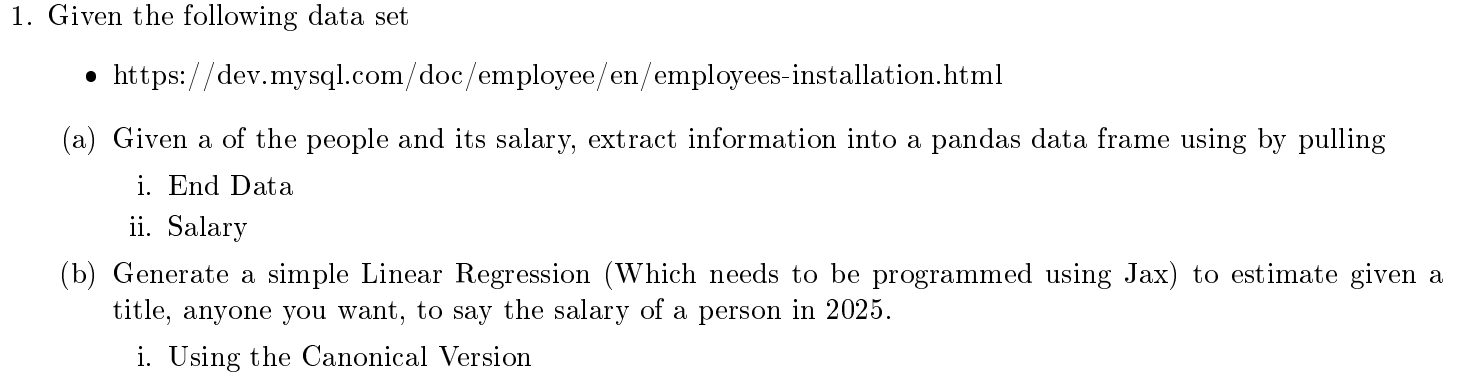
\includegraphics[width=1\textwidth]{screenshot001}
\end{figure}

\begin{lstlisting}
	import pandas as pd
	from sqlalchemy import create_engine
	import jax.numpy as jnp
	from jax import grad, jit
	import numpy as np
	
	def create_or_define_dataframes():
	# Replace with your database credentials and details
	username = 'root'
	password = ''
	host = 'localhost'
	database = 'employees'
	
	# Create the connection string
	connection_string = f'mysql+pymysql://{username}:{password}@{host}/{database}'
	
	# Create the connection engine
	engine = create_engine(connection_string)
	
	# Define the query
	query = 'SELECT * FROM salaries WHERE to_date != "9999-01-01" ORDER BY from_date DESC'
	
	# Execute the query and load the data into a pandas DataFrame
	df = pd.read_sql(query, engine)
	
	# Return the DataFrame
	return df
	
	def perform_linear_regression(df):
	# Extract year from from_date
	df['year'] = pd.to_datetime(df['from_date']).dt.year
	
	# Drop rows with missing values
	df = df.dropna(subset=['year', 'salary'])
	
	# Prepare the data for regression
	X = jnp.array(df['year'].values)
	y = jnp.array(df['salary'].values)
	
	# Normalize the data
	X_mean = jnp.mean(X)
	X_std = jnp.std(X)
	y_mean = jnp.mean(y)
	y_std = jnp.std(y)
	X = (X - X_mean) / X_std
	y = (y - y_mean) / y_std
	
	# Initialize parameters
	theta = jnp.array([0.0, 0.0])
	
	# Define the model
	def model(theta, x):
	return theta[0] + theta[1] * x
	
	# Define the loss function
	def loss_fn(theta, x, y):
	predictions = model(theta, x)
	return jnp.mean((predictions - y) ** 2)
	
	# Compute the gradient of the loss function
	grad_loss_fn = jit(grad(loss_fn))
	
	# Training loop
	learning_rate = 0.001
	num_iterations = 5000
	for _ in range(num_iterations):
	gradients = grad_loss_fn(theta, X, y)
	theta = theta - learning_rate * gradients
	
	# Predict the salary for the year 2025
	year_2025 = (jnp.array([2025]) - X_mean) / X_std
	predicted_salary = model(theta, year_2025)
	
	# Denormalize the prediction
	predicted_salary = predicted_salary * y_std + y_mean
	
	return predicted_salary[0]
	
	# Answeer
	df_salaries = create_or_define_dataframes()
	predicted_salary_2025 = perform_linear_regression(df_salaries)
	print(f"Predicted salary for the year 2025: {predicted_salary_2025}")
\end{lstlisting}

OUTPUT:

\begin{lstlisting}
	Predicted salary for the year 2025: 93926.453125
\end{lstlisting}

\begin{figure}[H]
	\centering
	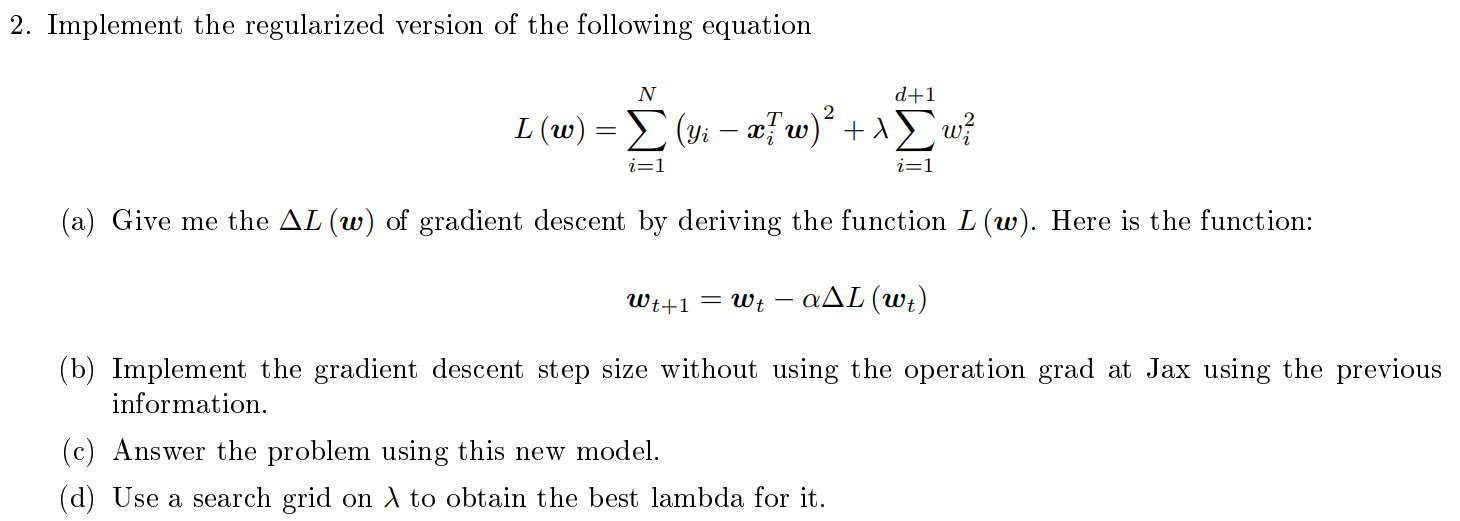
\includegraphics[width=1\textwidth]{screenshot002}
\end{figure}

Se esta trabajando, adjuntare el archivo bien hecho en unas horas

\begin{figure}[H]
	\centering
	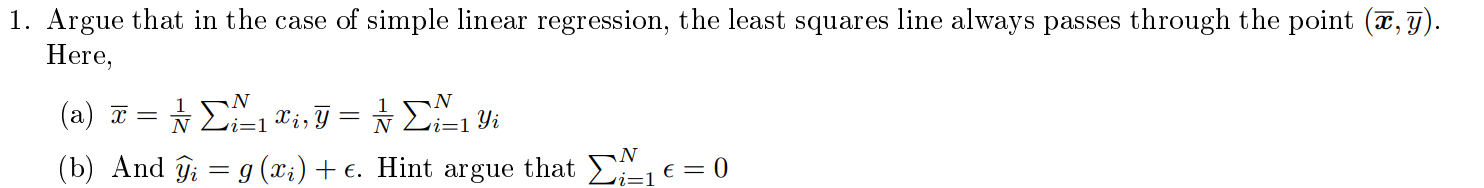
\includegraphics[width=1\textwidth]{screenshot003}
\end{figure}

% Respuesta 1
\section*{Respuesta 1}
La línea de mínimos cuadrados siempre pasa por el punto promedio \((x, y)\). Esto se puede demostrar de la siguiente forma:

\begin{itemize}
	\item Se define el promedio de \(x\) y \(y\) como:
	\[
	x = \frac{1}{N} \sum_{i=1}^N x_i, \quad y = \frac{1}{N} \sum_{i=1}^N y_i
	\]
	\item En regresión lineal, cada valor \(y_i\) puede expresarse como:
	\[
	y_i = g(x_i) + \epsilon
	\]
	Donde \(g(x_i)\) es la parte ajustada por el modelo y \(\epsilon\) es el error. Por definición, los errores cumplen:
	\[
	\sum_{i=1}^N \epsilon = 0
	\]
	\item Como los errores promedian a cero, el modelo pasa por el punto promedio \((x, y)\).
\end{itemize}

% Respuesta 2
\section*{Respuesta 2}
El coeficiente de determinación \(R^2\) es igual al cuadrado de la correlación entre \(X\) y \(Y\). Esto se puede demostrar usando las siguientes definiciones:

\begin{itemize}
	\item La correlación entre \(X\) y \(Y\) está dada por:
	\[
	\text{cor}(X, Y) = \frac{\text{Cov}(X, Y)}{\sqrt{\text{Var}(X) \cdot \text{Var}(Y)}}
	\]
	\item \(R^2\) se define como:
	\[
	R^2 = 1 - \frac{\text{Suma de Cuadrados de los Residuos (SSR)}}{\text{Suma Total de Cuadrados (SST)}}
	\]
	\item En el caso centrado (\(x = y = 0\)), se demuestra que:
	\[
	R^2 = \left( \text{cor}(X, Y) \right)^2
	\]
\end{itemize}


\begin{figure}[H]
	\centering
	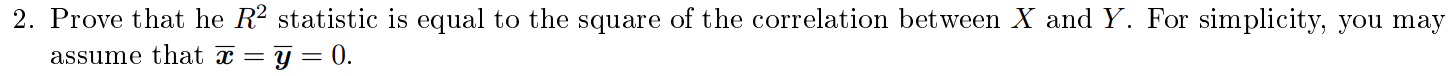
\includegraphics[width=1\textwidth]{screenshot004}
\end{figure}

% Respuesta 3
\section*{Respuesta 3}
Las principales diferencias entre KNN clasificador y regresor son las siguientes:

\begin{itemize}
	\item \textbf{KNN Clasificador:}
	\begin{itemize}
		\item Resuelve problemas de clasificación.
		\item Asigna la clase más frecuente entre los \(k\) vecinos más cercanos.
		\item La salida es una etiqueta categórica.
	\end{itemize}
	
	\item \textbf{KNN Regresor:}
	\begin{itemize}
		\item Resuelve problemas de regresión.
		\item Calcula el promedio de los valores de los \(k\) vecinos más cercanos.
		\item La salida es un valor continuo.
	\end{itemize}
\end{itemize}


\begin{figure}[H]
	\centering
	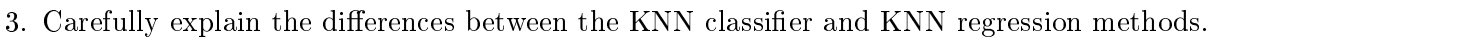
\includegraphics[width=1\textwidth]{screenshot008}
\end{figure}

\begin{figure}[H]
	\centering
	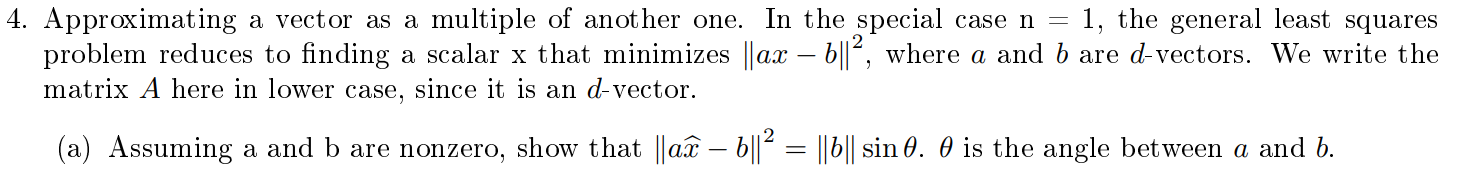
\includegraphics[width=1\textwidth]{screenshot006}
\end{figure}

% Respuesta 4
\section*{Respuesta 4}
Dado un escalar \(x\), se busca minimizar \(\|ax - b\|^2\), donde \(a\) y \(b\) son vectores.

\begin{itemize}
	\item En este caso, se demuestra que el error relativo está dado por:
	\[
	\|b - a\hat{x}\|^2 = \|b\|^2 - (\|b\| \cos \theta)^2 = \|b\|^2 \sin^2 \theta
	\]
	\item Por lo tanto:
	\[
	\|a\hat{x} - b\| = \|b\| \sin \theta
	\]
	Donde \(\theta\) es el ángulo entre \(a\) y \(b\). Esto muestra que el error depende del ángulo entre los vectores.
\end{itemize}


\begin{figure}[H]
	\centering
	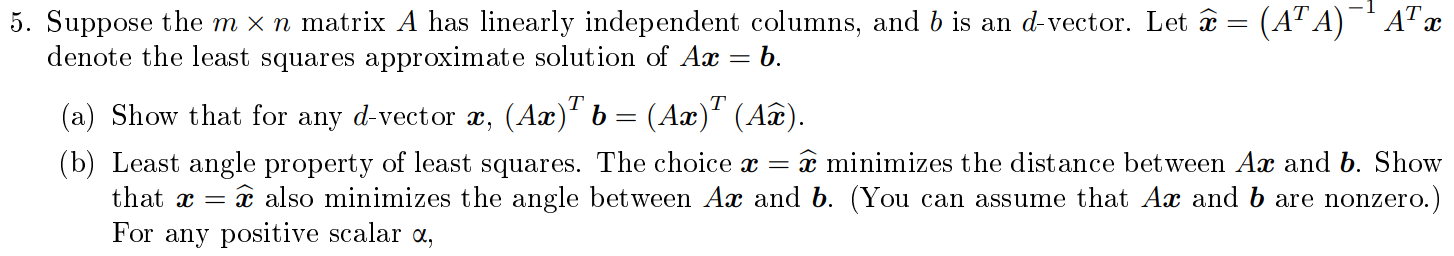
\includegraphics[width=1\textwidth]{screenshot007}
\end{figure}

% Respuesta 5
\section*{Respuesta 5}

Dada la solución de mínimos cuadrados:
\[
\hat{x} = \left( A^T A \right)^{-1} A^T b
\]

\begin{itemize}
	\item (a) Se demuestra que:
	\[
	(Ax)^T b = (Ax)^T (A\hat{x})
	\]
	Esto se debe a que \(\hat{x}\) minimiza la distancia entre \(Ax\) y \(b\), lo cual implica que:
	\[
	b^T (Ax - A\hat{x}) = 0
	\]
	
	\item (b) La solución \(\hat{x}\) también minimiza el ángulo entre \(Ax\) y \(b\). Esto se debe a que \(\hat{x}\) es la proyección ortogonal de \(b\) en el subespacio generado por las columnas de \(A\).
\end{itemize}


\printbibliography
\end{document}	

